Pour cette première partie, aucune justification n'est demandée et une seule réponse est possible par question.

Pour chaque question, reportez son numéro sur votre copie et indiquez votre réponse.

Une réponse fausse ou l'absence de réponse n'enlève aucun point.

\subsubsection*{Question 1}
Le nombre $\dfrac{1}{3} \times \dfrac{6}{5}-\dfrac{1}{5}$ est égal à :

\begin{center}
\begin{tabularx}{\linewidth}{*{4}{X}}
\textbf{A.~~} $\dfrac13$ &\textbf{B.~~} $\dfrac{5}{10}$ &\textbf{C.~~} $\dfrac15$ &\textbf{D.~~} $\dfrac53$\\
\end{tabularx}
\end{center}

\subsubsection*{Question 2}

Dans l'ensemble des nombres réels, l'équation $3 x+2= -5 x+4$ a pour solution :

\begin{center}
\begin{tabularx}{\linewidth}{*{4}{X}}
\textbf{A.~~} $x = - 1$ &\textbf{B.~~} $x = - 6$ &\textbf{C.~~} $x= \dfrac14$ &\textbf{D.~~} $x = 4$\\
\end{tabularx}
\end{center}

\subsubsection*{Question 3}
Pour tout nombre réel $x$, \quad$(2x -3)(2x + 3)$ \quad est égal à :

\begin{center}
\begin{tabularx}{\linewidth}{*{4}{X}}
\textbf{A.~~} $2x^2 - 9$&\textbf{B.~~}$2x^2-6$&\textbf{C.~~}$4x^2- 12x + 9$&
\textbf{D.~~}$4x^2 - 9$\\
\end{tabularx}
\end{center}

\subsubsection*{Question 4}
Dans un parc animalier, on compte 20 singes, ce qui représente $5 \%$ de l'effectif total des animaux de ce parc.

L'effectif total des animaux du parc animalier est égal à :

\begin{center}
\begin{tabularx}{\linewidth}{*{4}{X}}
\textbf{A.~~} \np{4000}&\textbf{B.~~} 400&\textbf{C.~~} \np{1000}& \textbf{D.~~} 100
\end{tabularx}
\end{center}

\subsubsection*{Question 5}
Une voiture parcourt une distance de 30 km à une vitesse moyenne de $\np[km/h]{60}$.

La durée du trajet, en minutes, est égale à :

\begin{center}
\begin{tabularx}{\linewidth}{*{4}{X}}
\textbf{A.~~} 30 &\textbf{B.~~} 60&\textbf{C.~~} 120&\textbf{D.~~} 18\\
\end{tabularx}
\end{center}

\subsubsection*{Question 6}

Une entreprise augmente sa production de $5\,\%$ par an.

Après 3 ans, la production initiale a été multipliée par :

\begin{center}
\begin{tabularx}{\linewidth}{*{4}{X}}
\textbf{A.~~} 1,15 &\textbf{B.~~} $1,05^{3}$&\textbf{C.~~} $3 \times 1,05$&\textbf{D.~~} $0,05^{3}$\\
\end{tabularx}
\end{center}

\subsubsection*{Question 7}

Dans le repère du plan ci-dessous, on a tracé la droite $(d)$.


\begin{center}

\psset{unit=1cm,arrowsize=2pt 3}
\begin{pspicture*}(-0.9,-1.5)(7,3)
\psaxes[linewidth=1.25pt,labelFontSize=\scriptstyle]{->}(0,0)(-0.9,-1.5)(6.9,2.9)
\psgrid[gridlabels=0pt,subgriddiv=1,gridwidth=0.15pt]
\psplot[plotpoints=500,linewidth=1.25pt,linecolor=blue]{-1}{7}{x 0.25 mul 1 sub}
\uput[u](6.5,0.6){\blue $(d)$}\uput[d](6.6,0){$x$}\uput[l](0,2.7){$y$}
\end{pspicture*}











\end{center}

L'équation réduite de la droite $(d)$ est :

\begin{center}
\begin{tabularx}{\linewidth}{*{4}{X}}
\textbf{A.~~} $y=4 x-1$&
\textbf{B.~~} $y=\dfrac{1}{4} x - 1$&
\textbf{C.~~} $y=x-\dfrac{1}{4}$&
\textbf{D.~~} $y=\dfrac{1}{4} x + 1$
\end{tabularx}
\end{center}

\subsubsection*{Question 8}

On considère une fonction $f$ définie sur $[-2~;~3]$, dont la courbe représentative est donnée ci-dessous.

\begin{minipage}{0.41\linewidth}
On peut dire que :

\medskip

\textbf{A.~~}$f$ est croissante sur $[-2~;~0]$

\textbf{B.~~} $f$ est positive sur $[-2~;~0]$

\textbf{C.~~} $f$ est décroissante sur $[0~;~3]$

\textbf{D.~~} $f$ est négative sur $[0~;~3]$
\end{minipage}\hfill
\begin{minipage}{0.56\linewidth}









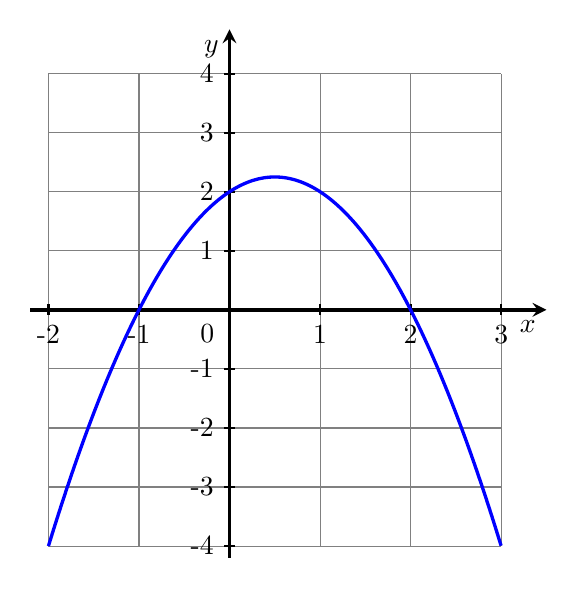
\begin{tikzpicture}[x=1.15cm,y=0.75cm,> = stealth]
	\draw[xstep=1, ystep=1,gray,thin,] (-2,-4) grid (3,4);
	\draw[line width=1.2pt,->](-2.2,0) -- (3.5,0) node[below left] {$x$};
	\draw[line width=1.2pt,->](0,-4.2) -- (0,4.75) node[below left] {$y$};
	\foreach \x in {-2,-1,1,2,3}{\draw[thick] (\x,2pt)--(\x,-2pt) node[below]{\np{\x}};}
	\foreach \y in {-4,...,-1,1,2,3,4}{\draw[thick] (2pt,\y)--(-2pt,\y) node[left]{\np{\y}};}
	\node[below left] at (-2pt,-2pt) {0};
	\draw[line width=1.2pt,color=blue,smooth,samples=100,domain= -2:3 ] plot(\x,{-(\x+1)*(\x-2)}) ;
\end{tikzpicture}
\end{minipage}
